%\documentclass[notes=show]{beamer} 
\documentclass[]{beamer}
\usetheme{umbc1}  
\useoutertheme{umbcfootline}
\setbeamertemplate{navigation symbols}{}  % see Remark below 
\setfootline{\insertshortauthor \hfill \insertsubtitle
    \hfill slide \insertframenumber/\inserttotalframenumber} 


\title{Bachelorarbeit}
\subtitle{Indentifikation von fehlerbehafteten Daten zur energiebewu\ss ten Programmierung}
\author[R. Frank]{Ren\'{e} Frank}
\institute[Ren\'{e} Frank]{
  Philipps-Universit\"at Marburg\\ 
  FB Mathematik \& Informatik\\[1ex]
  \texttt{frank@mathematik.uni-marburg.de}
}
\date{\today}

\usepackage[T1]{fontenc}
\usepackage[utf8]{inputenc}
\usepackage[ngerman]{babel}

%% use of boxes
\usepackage{fancybox}
\useinnertheme{umbcboxes}
\setbeamercolor{umbcboxes}{bg=violet!15,fg=black}

%% paste grafics
\usepackage{graphics}

%% tikz
\usepackage{tikz}
\usetikzlibrary{arrows,shadows,patterns} % for pgf-umlsd

%% framed
\usepackage{framed}


%% color package
\usepackage{color}

%% dashrule
\usepackage{dashrule}

%% different font family
\usepackage{helvet} %

%% listing
\usepackage{listings}

%% uml
\usepackage{uml}


%% set the items after \pause of one slide transparent 
\setbeamercovered{transparent}

\newcommand{\dashrule}[0]{\hdashrule{\linewidth}{1pt}{3pt}}

\newcommand{\partPage}[1]{
	{
	\setbeamertemplate{background canvas}{%
	\begin{tikzpicture}
    		\clip (0,0) rectangle (\paperwidth,\paperheight);
    		\fill[color=tmpBlue] (\paperwidth-10pt,0) rectangle (\paperwidth,\paperheight);
	\end{tikzpicture}}
	#1
	}
}

\defbeamertemplate*{part page}{borstel}[1][]{ 
 
  \begin{centering}
    \vskip1em\par
    \begin{beamercolorbox}[sep=8pt,center,#1]{}
      	\begin{myblock}
      		\usebeamerfont{part title}\usebeamercolor*[fg]{part name}\insertpart\par
      	\end{myblock}
    \end{beamercolorbox}
  \end{centering}
} 
\setbeamertemplate{part page}[borstel][]

\definecolor{llightGray}{HTML}{C0C0C0}
\definecolor{Sand}{HTML}{FFFFCC}
\definecolor{LLightBlue}{HTML}{CCCCFF}
\definecolor{LLila}{HTML}{870055}
\definecolor{DarkGrey}{rgb}{0.1,0.1,0.1}
\definecolor{tmpBlue}{HTML}{9999D9}

\newtheorem{mydef}{Strategien}

\newsavebox\blockbox
\newenvironment{myblock}{%
  \begin{lrbox}{\blockbox}%
    \begin{minipage}{.8\textwidth}
}{
    \end{minipage}
  \end{lrbox}
  \tikz\node[
    draw=black,
    line width=0.5pt,
    inner sep=10pt,
    outer sep=0pt,
  ]{\usebox\blockbox};
}

\lstdefinestyle{stJava}{basicstyle=\scriptsize\ttfamily,
	classoffset=0,	
	numbers=left, 				% show line numbers on the left
	stepnumber=1, 				% show every  line number
	numberstyle=\scriptsize, 			% font sitze of line numbers
	numbersep=5pt, 				% separation to the text
	language=Java,				% language of source
	backgroundcolor={\color{Sand}},
	stringstyle=\color{blue},		% style of strings
	emphstyle=\color{red},			% sytle of ???
	commentstyle=\color{gray},		% style of comments
	keywordstyle=\bfseries,			% style of keywords
	captionpos=b,
	tabsize=4,				% indentation
	showspaces=false,			% show spaces
	showtabs=false,				% show tabs
	showstringspaces=false,			% show spaces in strings
	breaklines=true,			% breaks long lines
	keywordstyle=\color{LLila},          % keyword style
	morekeywords={enum},
  	%stringstyle=\color{mauve},         % string literal style
  	escapeinside={\%*}{*)},           % if you want to add LaTeX within your code
  	classoffset=1,
	morekeywords={RANDOM, LOSS, ZERO, BITFLIP, BITFLIPB, NONE},keywordstyle=\color{blue},
	classoffset=0
	%frame=tbl 				% can be: none, single, trbl (or trBL, ...), shadowbox	      		
%    keywordstyle=\color{blue}\bfseries,
}

\begin{document}

%% Nummerierung sections
\setbeamertemplate{section in toc}[sections numbered]

\frame{
	\titlepage
}

\frame{
	\frametitle{Accuracy-Aware Data Processing}

	\begin{itemize}
		\item steigende Energiekosten
		\item immer höhere Rechenleistungen
		\item wachsende Zahl an Online-Services
	\end{itemize}

	\begin{minipage}{0.45\linewidth}
		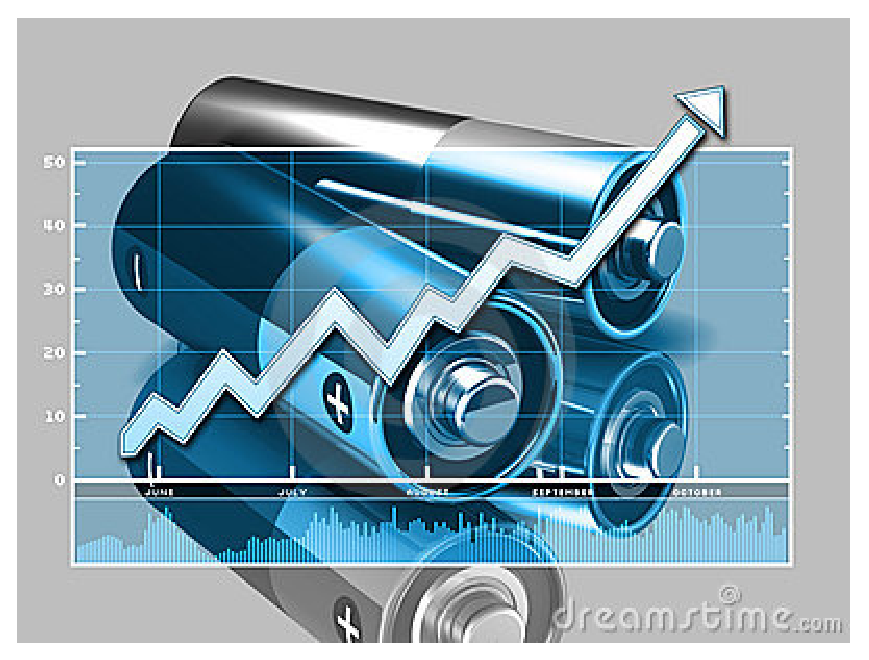
\includegraphics[scale=0.25]{graphics/energycons.eps}
	\end{minipage}
	\begin{minipage}{0.4\linewidth}
		
\includegraphics[scale=0.2]{graphics/cloud.eps}
	\end{minipage}	

	Accuracy-Aware Data Processing
	\begin{itemize}
		\item fehlertoleranz ausnutzen
		\item Fehlerfreiheit und Genauigkeit reduzieren
	\end{itemize}	
	
	\vfill
\begin{tiny}
	Quelle Bild 1: http://www.dreamstime.com/ - Zugriff: 15.10.12\\[-0.2cm]
	Quelle Bild 2: http://gsablogs.gsa.gov/gsablog/files/2012/09/Cloud-computing-9-25-12b.jpg - Zugriff: 15.10.12
\end{tiny}
}


%% ---------------------------------------------------------------------------------------------

\part{Motivation/Zielsetzung}
\partPage{
\frame[plain]{\partpage}
}


\frame{
	
	\frametitle{Fehlerinjektion für Datenströme}	
	
	\begin{itemize}
		\item Fehlerinjektion minimal-invasiv
		\note[item]{d.h. mit möglichst wenig Änderungen im Code vornehmen zu müssen}   
		\item<2-> Nur einen minimalen Overhead erzeugen
		\note[item]{um die Verwendung für große verteilte Systeme (z.B. Hadoop), bei denen neben der Fehlerinjektion zugleich Energiemessungen vorgenommen werden können, zu ermöglichen.} 
		\item<3-> Alle Arten von Datenströmen sollten berücksichtigt werden
		\note[item]{weil für ``Accuracy Awareness'' sowohl modifizierte Disk- als auch Network-Hardware simuliert werden soll.}   
		\item<4-> Eine dynamische Regulierung der Fehlerwerte zur Laufzeit
	\end{itemize}
}

%% ---------------------------------------------------------------------------------------------

\part{Design/Implementierung}
\partPage{
\frame[plain]{\partpage}


}

\frame{
	\frametitle{Funktionen}
	\hspace*{-0.5cm}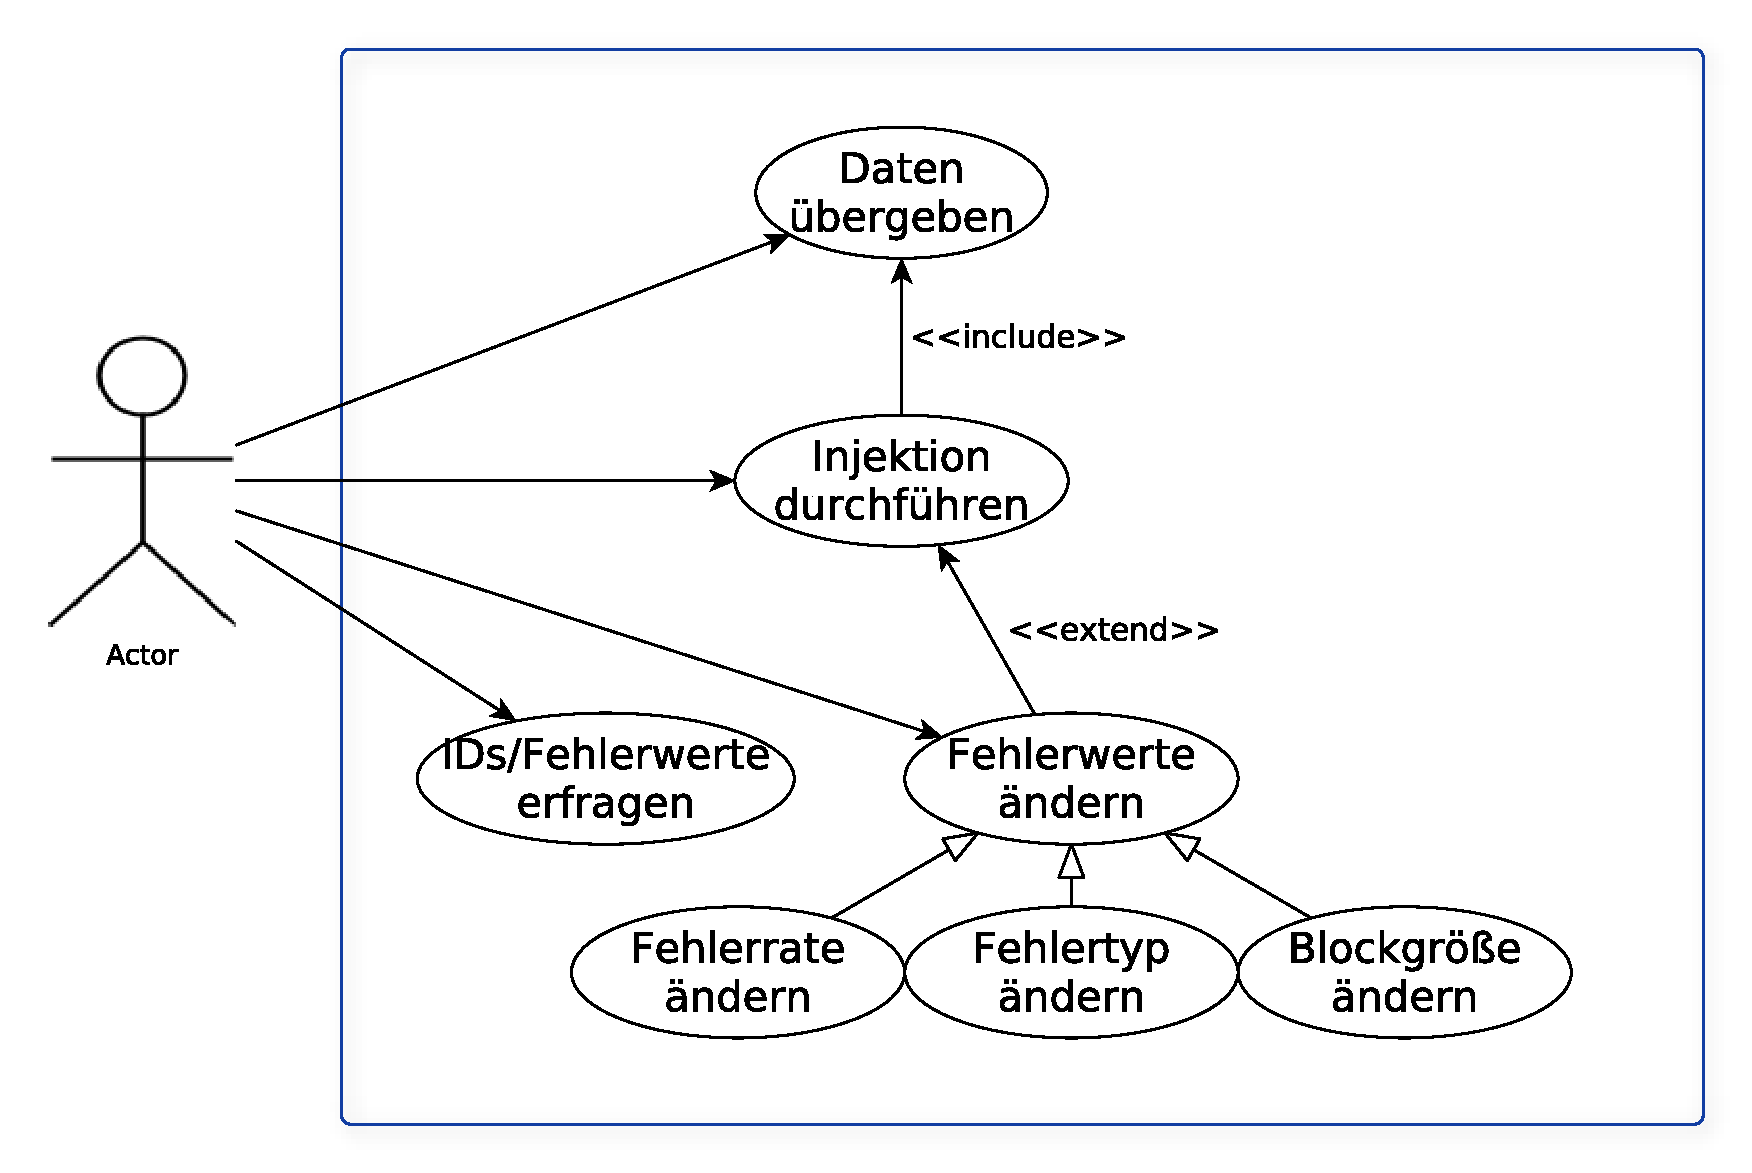
\includegraphics[scale=0.4]{graphics/Anwendungsfalldiagramm2.eps}
}

\frame{
	\frametitle{Wichtige Klassen}
	\begin{itemize}
		\item<1> StreamProcesser
		\begin{itemize}
			\item Einlesen und Ausgabe der Daten, Start der Fehlerinjektion
		\end{itemize}
		\item<1> InjectionStrategy
		\begin{itemize}
			\item Oberklasse der Injektionsstrategien
		\end{itemize}	
		\item<1> AddRunTimeAnnotation
		\begin{itemize}
			\item Dynamische Modifikation der Annotationen
		\end{itemize}	
		\item<1> Controller
		\begin{itemize}
			\item Steurerung aller Funktionen
		\end{itemize}				
	\end{itemize}
}

\begin{frame}[fragile]
	\frametitle{StreamProcessor}

	Aufgaben
	\begin{itemize}
		\item Daten fehlerbehafteter Streams einlesen
		\begin{itemize}
			\item Fehlermarkierung durch Annotationen
				\lstinputlisting[style=stJava]{listings/FaultInj2.java}
		\end{itemize}
		\item als Byte-Liste zur Datenmanipulation an Klasse Context weitergeben
		\item manipulierte Daten holen und in entsprechender Form ausgeben
	\end{itemize}
	
\end{frame}


\begin{frame}[fragile]
	\frametitle{Fehlermarkierung}

	\begin{itemize}
		\item id muss eindeutig sein
		\item type muss vorhanden sein
		\item rate liegt zwischen 0 und 1
	\end{itemize}

	\lstinputlisting[style=stJava]{listings/FileProcessor1.java}
\end{frame}


\frame{

\begin{figure}[!htb] 
\begin{scriptsize}

\centering
		\umlDiagram[box=,border, sizeX=9cm,sizeY=6cm,ref=pack]{		
			\umlClass[pos=\umlTop{pack}, stereotype=Class, posDelta={0, -7},
				refpoint=t]{StreamProcessor}{}{}
			\umlClass[pos=\umlTop{pack}, stereotype=Class, posDelta={0, -1},
				refpoint=t]{Context}{}{}
			\umlClass[pos=\umlTopRight{pack}, stereotype=Abstract Class, posDelta={-6,-1},
				refpoint=t]{InjectionStrategy}{}{}	
			\umlClass[pos=\umlLeft{pack}, stereotype=Class, posDelta={4, 1},
				refpoint=t]{Reducer}{}{}	
			\umlClass[pos=\umlRight{pack}, stereotype=Annotation, posDelta={-5, 1},
				refpoint=t]{FaultInj}{}{}
			\umlClass[pos=\umlBottom{pack}, stereotype=Annotation, posDelta={0, 3.5},
				refpoint=t]{FaultInjects}{}{}																	\umlInner{Reducer}{StreamProcessor}
			\umlInstance{StreamProcessor}{FaultInj}	
			\umlInstance{StreamProcessor}{FaultInjects}
			\umlInstance{StreamProcessor}{Context}
			\umlInstance{Context}{InjectionStrategy}									
		}% End of diagram
	\end{scriptsize}
\end{figure}	
}

\frame{
	\frametitle{Wichtige Klassen}
	\begin{itemize}
		\item<1> StreamProcesser
		\begin{itemize}
			\item Einlesen und Ausgabe der Daten, Start der Fehlerinjektion
		\end{itemize}
		\item<2> InjectionStrategy
		\begin{itemize}
			\item Oberklasse der Injektionsstrategien
		\end{itemize}	
		\item<0> AddRunTimeAnnotation
		\begin{itemize}
			\item Dynamische Modifikation der Annotationen
		\end{itemize}	
		\item<0> Controller
		\begin{itemize}
			\item Steurerung aller Funktionen
		\end{itemize}				
	\end{itemize}
}

\frame{
	\frametitle{InjectionStrategy}
	
	\begin{itemize}
		\item abstrakte Oberklasse aller Strategien
		\item keine eigene Injektionslogik $\rightarrow$ abstrakte Methode
		\item Zufallsfunktion zur Fehlerinjektion
		\begin{itemize}
			\item entscheidet anhand Fehlerrate über Injektion
		\end{itemize}
	\end{itemize}
	
	\begin{mydef}
		\begin{itemize}
			\item Bitflip
			\item BitflipB
			\item Random
			\item Loss
			\item Zero
		\end{itemize}
	\end{mydef}		
}

\frame{
\begin{figure}[!htb] 
	\begin{scriptsize}
\centering
		\umlDiagram[box=,border,sizeX=9cm,sizeY=8cm,ref=pack]{	
			\umlClass[pos=\umlTop{pack}, stereotype=Class, posDelta={0, -1},
				refpoint=t]{Context}{}{}	
			\umlClass[pos=\umlTop{pack}, stereotype=Abstract Class, posDelta={0, -6},
				refpoint=t]{InjectionStrategy}{
					\umlAttribute[visibility=\# , type=FaultValue{[]}]{faults}				
				}{
					\umlMethod[visibility=+, type=void]{\textit{runInjection}}{}
					\umlMethod[visibility=\# , type=boolean]{isInject}{double}				
				}
			\umlClass[pos=\umlLeft{pack}, stereotype=Class, posDelta={6, -2},
				refpoint=t]{StrategyBitflip}{}{
					\umlMethod[visibility=+, type=void]{runInjection}{}				
				}
			\umlClass[pos=\umlRight{pack}, stereotype=Class, posDelta={-6, -2},
				refpoint=t]{StrategyRandom}{}{
					\umlMethod[visibility=+, type=void]{runInjection}{}					
				}	
			\umlClass[pos=\umlBottom{pack}, stereotype=Class, posDelta={0, 4},
				refpoint=t]{...}{}{
					\umlMethod[visibility=+, type=void]{runInjection}{}					
				}				
			\umlInstance{Context}{InjectionStrategy}									
			\umlSubclass{InjectionStrategy}{StrategyBitflip}	
			\umlSubclass{InjectionStrategy}{StrategyRandom}
			\umlSubclass{InjectionStrategy}{...}											
		}% End of diagram
	\end{scriptsize}
\end{figure}
}

\begin{frame}[fragile]
	\frametitle{Strategieauswahl}

		\lstinputlisting[style=stJava]{listings/injektionFolie.java}
\end{frame}

\frame{
\frametitle{Wichtige Klassen}
	\begin{itemize}
		\item<0> StreamProcesser
		\begin{itemize}
			\item Einlesen und Ausgabe der Daten, Start der Fehlerinjektion
		\end{itemize}
		\item<1> InjectionStrategy
		\begin{itemize}
			\item Oberklasse der Injektionsstrategien
		\end{itemize}	
		\item<2> AddRunTimeAnnotation
		\begin{itemize}
			\item Dynamische Modifikation der Annotationen
		\end{itemize}	
		\item<0> Controller
		\begin{itemize}
			\item Steurerung aller Funktionen
		\end{itemize}				
	\end{itemize}
}

\frame{
	\frametitle{AddRunTimeAnnotation}

	\vspace{-0.1cm}	
	
	\begin{minipage}{4cm}
		\begin{itemize}
			\item Library Javassist
			\item Manipulation der Annotationen
			\item reload der Class-Datei
		\end{itemize}
	\end{minipage}
	\begin{minipage}{4cm}
	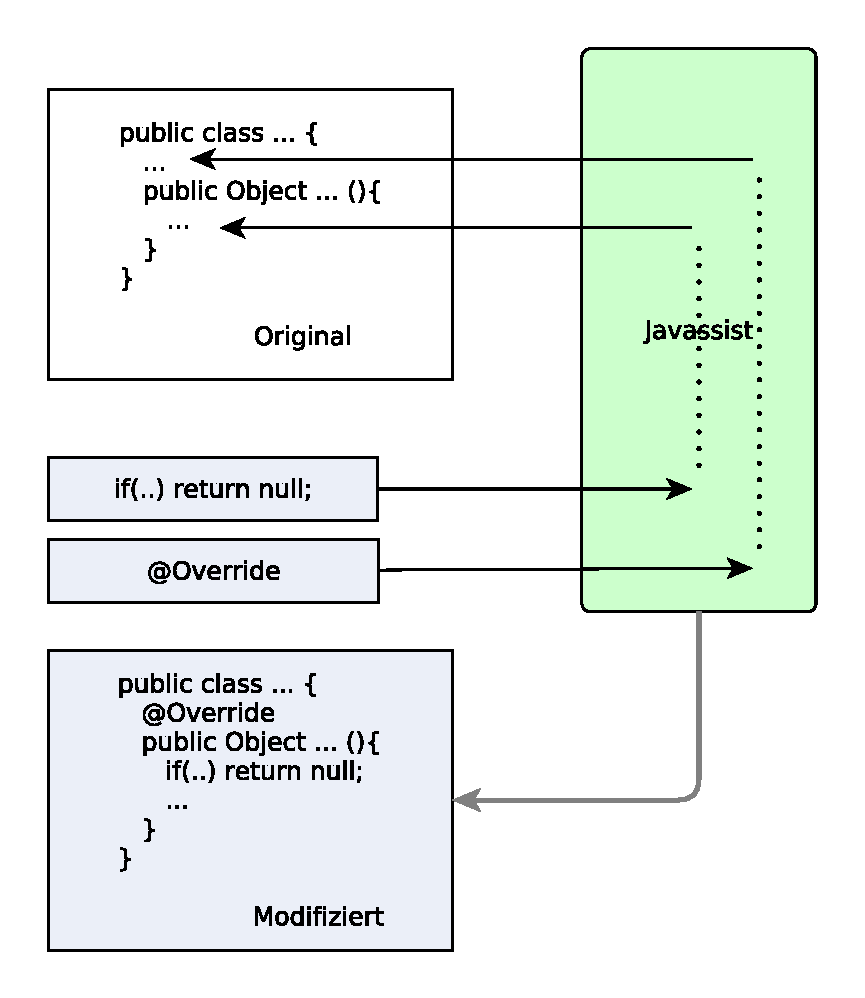
\includegraphics[scale=0.475]{graphics/javassist.eps}
	\end{minipage}	
	
	\begin{tiny}
	Quelle: http://www.sciencedirect.com/science/article/pii/S0164121211000501 - Zugriff: 15.10.12
	\end{tiny}
}

\begin{frame}[fragile]
	\frametitle{Bestimmung der zu manipulierenden Streams}
	
	\begin{itemize}
		\item Ct = comile-time
		\item cc vom Typ CtClass 
	\end{itemize}

	\lstinputlisting[style=stJava]{listings/AddRuntime2.java}
\end{frame}

\begin{frame}[fragile]
	\frametitle{Anlegen neuer Annotationen}
	
	\begin{itemize}
		\item Unterscheidung FaultInj und FaultInjects
		\item anlegen der entsprechenden Annotation in Annotation-Array
	\end{itemize}

	\lstinputlisting[style=stJava]{listings/AddRuntime4.java}
\end{frame}

\begin{frame}[fragile]
	\frametitle{Hinzufügen der Fehlerwerte zu FaultInjects}
	
	\begin{itemize}
		\item \textit{fis} = Array mit Fehlerwerte eines markierten Streams
	\end{itemize}

	\lstinputlisting[style=stJava]{listings/AddRuntime5Folie.java}
\end{frame}

\begin{frame}[fragile]
	\frametitle{Laden der Klasse mit neuen Annotationen}
	
	\begin{itemize}
		\item ctClass zu normaler Class Datei umwandeln
		\item javassist.util.HotSwapper $\rightarrow$ Bytecode reload
	\end{itemize}

	\lstinputlisting[style=stJava]{listings/AddRuntime6.java}
\end{frame}

%\frame{
%\begin{figure}[!htb]
%	\begin{scriptsize}
%\centering
%		\umlDiagram[box=,border,sizeX=10cm,sizeY=6cm,ref=pack]{		
%			\umlClass[pos=\umlTop{pack}, stereotype=Class, posDelta={0, -1},
%				refpoint=t]{AddRunTimeAnnotation}{}{}
%			\umlClass[pos=\umlBottomLeft{pack}, stereotype=Class, posDelta={5, 5},
%				refpoint=t]{FileProcessor}{}{}
%			\umlClass[pos=\umlTopRight{pack}, stereotype=Annotation, posDelta={-5, -5},
%				refpoint=t]{FaultInj}{}{}	
%			\umlClass[pos=\umlBottomRight{pack}, stereotype=Annotation, posDelta={-5, 5},
%				refpoint=t]{FaultInjects}{}{}
%			\umlClass[pos=\umlBottom{pack}, stereotype=class, posDelta={0, 5},
%				refpoint=t]{Controller}{}{}		
%			\umlInstance{AddRunTimeAnnotation}{FaultInj}	
%			\umlInstance{AddRunTimeAnnotation}{FaultInjects}
%			\umlInstance{Controller}{FileProcessor}
%			\umlInstance{AddRunTimeAnnotation}{FileProcessor}									
%		}% End of diagram
%	%	\captionsetup{list=false}
% 		\end{scriptsize}
%\end{figure}
%}


\frame{
\frametitle{Wichtige Klassen}
	\begin{itemize}
		\item<0> StreamProcesser
		\begin{itemize}
			\item Einlesen und Ausgabe der Daten, Start der Fehlerinjektion
		\end{itemize}
		\item<0> InjectionStrategy
		\begin{itemize}
			\item Oberklasse der Injektionsstrategien
		\end{itemize}	
		\item<1> AddRunTimeAnnotation
		\begin{itemize}
			\item Dynamische Modifikation der Annotationen
		\end{itemize}	
		\item<2> Controller
		\begin{itemize}
			\item Steurerung aller Funktionen
		\end{itemize}				
	\end{itemize}
}

\frame{
	\frametitle{Controller}
	\begin{itemize}
		\item Steuert alle Funktionalitäten
		\item Verwaltung der Funktionalitäten durch JMX-Agent
		\begin{itemize}
			\item Komponenten zur Laufzeit managen
			\item Anwendungsfunktionalität leichter administrierbar 
		\end{itemize}		  
		\item Schnittstelle MBeanController
		\begin{itemize}
			\item liefert dem Client Zugriff auf gegebene Funktionen
		\end{itemize}
	\end{itemize}
}


\frame{
	\frametitle{Controller/MBean}
	
		
	
	\begin{figure}[!htb]
	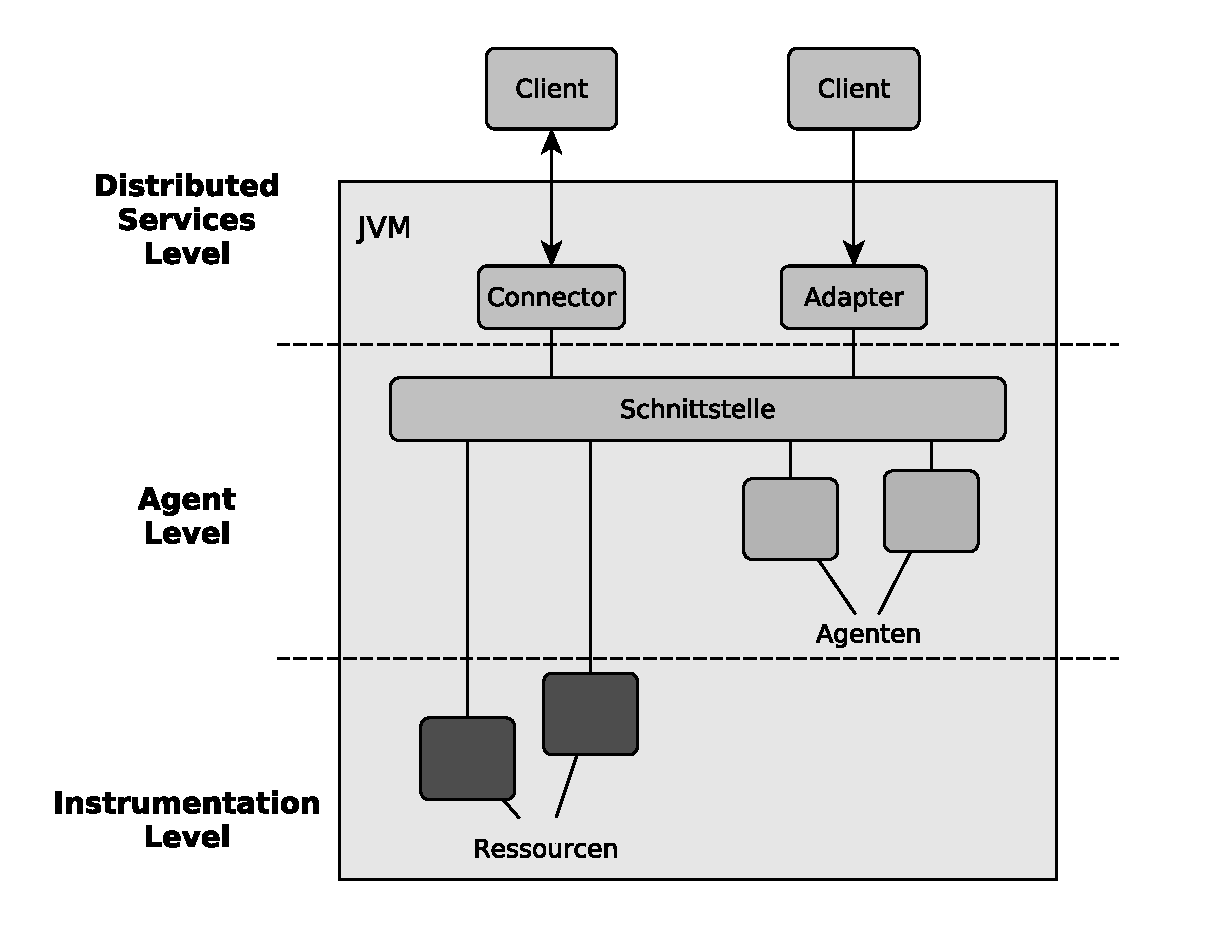
\includegraphics[scale=0.5]{graphics/JMX.eps}
	\end{figure}
		\vspace{-0.5cm}
	\begin{tiny}
	Quelle: http://de.wikipedia.org/wiki/Datei:Jmx\_ architektur.png - Zugriff: 15.10.12
	\end{tiny}
}


\begin{frame}[fragile]
	\frametitle{Schnittstelle zum MBeanServer}

	\begin{itemize}
		\item bereitgestellte Funktionalitäten
	\end{itemize}

	\lstinputlisting[style=stJava]{listings/Controller2Folie.java}
	
	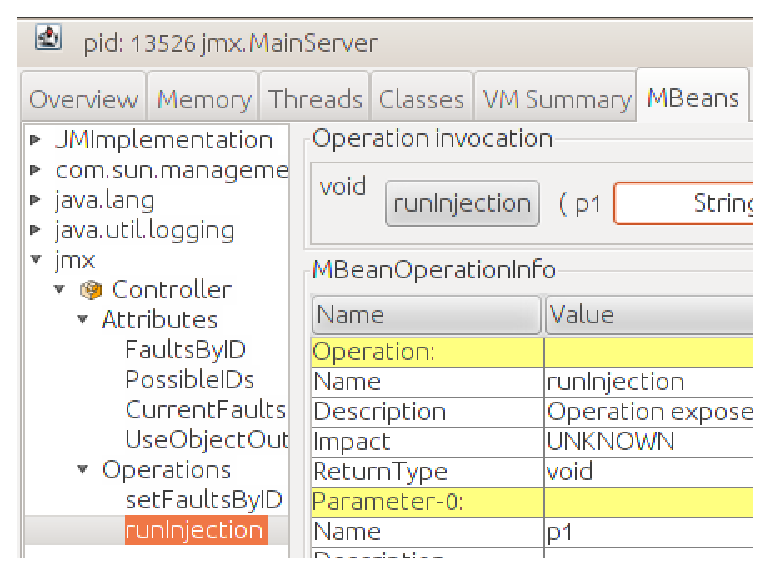
\includegraphics[scale=0.5]{graphics/client.eps}
\end{frame}

\begin{frame}[fragile]
	\frametitle{Verbindungsaufbau (1)}

	\lstinputlisting[style=stJava]{listings/Controller1.java}
\end{frame}

\begin{frame}[fragile]
	\frametitle{Verbindungsaufbau (2)}

	\lstinputlisting[style=stJava]{listings/Controller3.java}
\end{frame}

%% ---------------------------------------------------------------------------------------------


\end{document}

